\chapter{Organic Chemistry}

Organic chemistry is the study of complex carbon-based compounds. In ordinary level, students should become familiar with basic naming, properties, and reactions of simple organic compounds. This chapter presents a variety of activities to make these topics more hands-on and more connected to daily life.

\subsection{Alkanes}

Students first study alkanes, hydrocarbon chains of various length. Many alkanes are common in daily life and a useful activity is to present them to students to observe their properties.

\subsubsection*{Learning Objectives}
\begin{itemize}
\item{To observe common alkanes}
\item{To observe a correlation between chain length and state of matter in alkanes}
\end{itemize}

\subsubsection*{Materials}
Butane lighter (kibiriti cha gasi), petrol (mafuta ya gari), kerosene (mafuta ya taa), vaseline (mafuta ya kupaka), candle wax (mabaki ya mishumaa), pin or syringe needle

\subsubsection*{Preparation}
\begin{enumerate}
\item{Move some desks up to the chalk board. Place each of the above items (butane lighter, petrol, kerosene, vaseline, and candle wax) on the desks in this order.}
\item{On the chalk board, write approximate chemical formulas for each compound. Butane is \ce{C4H10}; petrol is \ce{C8H18}, kerosene is about \ce{C12H26}, vaseline is about \ce{C20H42}, and wax is about \ce{C25H52}. Note that these are only approximate formulas, especially for the larger molecules.}
\end{enumerate}

\subsubsection*{Activity Procedure}
\begin{enumerate}
\item{Comment on the states of matter of each of the materials.}
\item{Rank the samples from smallest molecules to largest.}
\item{Comment on the correlation between size of molecule and state of matter.}
\item{Use the pin or needle to press the release valve on the underside of the butane lighter. The sound of rushing gas should be heard. This is butane gas. \textit{Only release a small amount.}}
\end{enumerate}

\subsubsection*{Results and Conclusion}
Larger hydrocarbons tend to be solids while smaller hydrocarbons tend to be liquids. The smallest hydrocarbons (methane, ethane, propane, and butane) are gases at room temperature and atmospheric pressure.

\subsubsection*{Discussion Questions}
\begin{enumerate}
\item{Which substances have the strongest attraction between molecules? Which have the weakest? How do you know?}
\item{What is the connection between attraction between molecules and boiling point / melting point?}
\item{What is the connection between attraction between molecules and the size of hydrocarbon molecules?}
\item{Why is butane a liquid inside the lighter and a gas outside?}
\end{enumerate}

\subsubsection*{Notes}
The only forces of attraction between molecules of hydrocarbons are van der Waals forces or London dispersion forces. The strength of these forces increases with the size of the molecules. Therefore substances made from large hydrocarbon molecules (e.g. wax) have stronger intermolecular forces than those made from small hydrocarbon molecules (e.g. butane). The stronger the intermolecular forces, the greater thermal energy must be present to shake the molecules apart from each other, that is, to cause melting and boiling.
Butane is a gas at room temperature and atmospheric pressure. Butane lighters hold the butane under pressure to force the molecules together to form a liquid. This allows for more efficient storage of the butane. When the valve on the lighter is pressed, butane can exit the lighter where it vapourizes in the reduced pressure.

\subsection{Preparation of Ethanol by Fermentation of Sugar}

After learning about the simple hydrocarbons (alkanes, alkenes, and alkynes), students should learn about substituted hydrocarbons. Substituted hydrocarbons are simple hydrocarbons with functional groups. Functional groups are more reactive parts of organic molecules, usually involving atoms such as oxygen, nitrogen, sulphur, and the halogens. One of the functional groups is the hydroxyl group, -OH. Organic molecules with a hydroxyl group are called alcohols, e.g. methanol, ethanol, butanol.

In daily life, the most common of the alcohols is ethanol, \ce{CH3CH2OH}. Ethanol is a colourless liquid with a characteristic odour. Ethanol may be produced directly from petroleum but ethanol produced for human consumption is prepared by a biological process, the fermentation of carbohydrates. Fermentation is the chemical breakdown of a substance by bacteria, yeasts, or other micro-organisms. Yeast works on sugar to break it down into alcohol and carbon dioxide gas. Fermentation of starch or sugar produces many common alcoholic beverages, e.g. beer and wines.

The following activity may be used to show the preparation of ethanol by fermentation.

\subsubsection*{Learning Objectives}
\begin{itemize}
\item{To prepare ethanol in the laboratory}
\end{itemize}

\subsubsection*{Materials}
Gas generator*, spatula*, yeast, sugar, and lime water*.

\subsubsection*{Activity Procedure}
\begin{enumerate}

\item{Put 10-20~mL of lime water in a test tube and put the open end of the delivery tube from the gas generator into this solution.}
\item{Make a sugar solution by dissolving about 3 full spoonfuls of sugar into about 100 mL of water.}
\item{Put about 1 1/2 teaspoons of yeast into the sugar solution and seal the bottle.}
\item{Label the container and set it aside in a safe place. Come back each day to make observations about any change in appearance in the lime water.}
\item{After 3 days, write down observation about the appearance of the lime water.}
\item{Observe the appearance and smell of the solution remaining.}
\end{enumerate}

\subsubsection*{Results and Conclusion}
When yeast is added to the sugar solution and left for some time a gas is generated. The gas turns the limewater milky which confirms that it is carbon dioxide. The solution remaining in the bottle will have a faint smell of alcohol (pombe) which shows the presence of ethanol.

\subsubsection*{Clean Up Procedure}
\begin{enumerate}
\item{Gas generators can be collected and stored for later use.}
\item{Collect all the used materials, cleaning and storing items that will be used later. No special waste disposal is required.}
\end{enumerate}

\subsubsection*{Discussion Questions}
\begin{enumerate}
\item{What is the role of yeast in this experiment?}
\item{What happens to the lime water in this experiment? What does this indicate?}
\item{Where is this process applied in the village?}
\end{enumerate}

\subsubsection*{Notes}
If gas generators have been made in a previous experiment, these can be used here.

\subsection{Reaction of Ethanol with Oxygen}

One property of alcohols is that they readily combust. Ethanol burns readily in air with an almost colourless flame, producing carbon dioxide and water.

\subsubsection*{Learning Objectives}
\begin{itemize}
\item{To describe the properties of alcohols.}
\end{itemize}

\subsubsection*{Materials}
Colourless spirit, match box, soda cap with plastic removed or lid of jam jar, knife.

\subsubsection*{Hazards and Safety}
\begin{itemize}
\item{Ethanol is flammable and the flame is hot. This activity should not be done on or around plastic or cloth material. Advise students that the flame may be colourless, thus special care must be taken. An ethanol flame can be extinguished with water if needed.}
\end{itemize}

\subsubsection*{Activity Procedure}
\begin{enumerate}
\item{Put approximately 1 ml of ethanol into a soda bottle cap.}
\item{Light a match and touch it to the ethanol.}
\end{enumerate}

\subsubsection*{Results and Conclusion}
When the lit match was brought to the flame the ethanol burns in the presence of oxygen. A colourless flame will form. The balanced chemical equation for this reaction is
\begin{center}
\ce{C2H5OH(l) + 3O2(g) $$\longrightarrow$$ 3H2O(g) + 2CO2(g)}
\end{center}

\subsubsection*{Clean Up Procedure}
\begin{enumerate}
\item{Collect all the used materials, cleaning and storing items that will be used later. No special waste disposal is required.}
\end{enumerate}

\subsubsection*{Discussion Questions}
\begin{enumerate}
\item{Explain what happens when alcohol is lit with a match.}
\item{Write a balanced chemical equation for the combustion of ethanol.}
\item{This experiment would not have worked if you used beer, although it does contain some ethanol. Explain.}
\end{enumerate}

\subsection{Oxidation of Ethanol}

The oxidation of ethanol is a good example of a reaction in organic chemistry where one organic compound is converted into another. There are two methods for oxidizing ethanol that are viable in a simple laboratory - each are presented with an activity. The first activity shows the biological oxidation of ethanol to ethanoic (acetic) acid. This activity requires very little class time but the experiment itself may take many days. The second activity shows the chemical oxidation of ethanol to ethanal (acetaldehyde) with potassium permanganate. This activity is much faster, but the product is difficult to prove, and the reaction produces a very bad odour.

\subsection{Reaction of alcohol and carboxylic acid}

One organic reaction of major importance is esterification. Esterification is the formation of an ester (ROOR') group through the reaction of an alcohol and a carboxylic acid. Many esters are volatile and their production can be observed by smell.\\
This activity presents an opportunity for students to perform their own organic reaction. Ideally students perform this activity in pairs.

\subsubsection*{Learning Objectives}
\begin{itemize}
\item{To describe the reaction between spirit(ethanol) and citric acid}
\end{itemize}

\subsubsection*{Materials}
Citric acid powder*, methylated spirits*, battery acid (5~M sulphuric acid)*, beakers*, tea spoon.

\subsubsection*{Hazards and Safety}
\begin{itemize}
\item{Battery acid is 5~M sulphuric acid. Concentrated sulphuric acid is corrosive to the skin and clothes. Avoid contact with skin and eyes. Neutralize spills with bicarbonate of sodium (baking soda).}
\end{itemize}

\subsubsection*{Preparation}
\begin{enumerate}
\item{Make a saturated solution of citric acid and put in one of the beakers.}
\end{enumerate}

\subsubsection*{Activity Procedure}
\begin{enumerate}
\item{Take a small amount of the citric acid solution, about three water capfuls, and pour it in the second beaker.}
\item{Into the second beaker add about one capful of battery acid and mix.}
\item{To the mixture above add about three capfuls of spirit and mix. Observe the smell.}
\end{enumerate}

\subsubsection*{Results and Conclusion}
Spirit reacts like ethanol and reacted with citric acid in the presence of acidic medium to produce a ester with fragrant smell.

\subsubsection*{Clean Up Procedure}
\begin{enumerate}
\item{Collect all the used materials, cleaning and storing items that will be used later. No special waste disposal is required.}
\end{enumerate}

\subsubsection*{Discussion Questions}
\begin{enumerate}
\item{Why was battery acid added to the citric acid solution?}
\item{What smell did you detect in your experiment?}
\item{Can you tell what the product is? Write the chemical reaction equation assuming that the spirit contains only ethanol.}
\end{enumerate}

\subsubsection*{Notes}
Citric acid has three carboxylic acid groups. You might draw its structure for students on the board: 
\begin{center}
\begin{figure}[h]
\begin{center}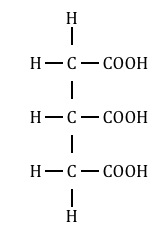
\includegraphics[scale=0.5]{img/citric-acid.pdf}\end{center}
\caption{Citric Acid}
\end{figure}
\end{center}


\subsection{Preparation of Soap}

An organic reaction of great practical value is saponification. Saponification is the reaction of a fatty acid with a strong base to form soap. The following activity is useful for demonstrating to students both an organic reaction with a dramatic result as well as explaining the manufacture of a common substance.

\subsubsection*{Learning Objectives}
\begin{itemize}
\item{To prepare a sample of soap from vegetable oil.}
\end{itemize}

\subsubsection*{Materials}
Sunflower oil (vegetable oil), caustic soda (sodium hydroxide)*, distilled water*, table salt (sodium chloride)*, jam jar, filter papers, heat source*, beaker*.

\subsubsection*{Hazards and Safety}
\begin{itemize}
\item{Sodium hydroxide (caustic soda) is corrosive to the skin and even in a dilute solution can blind. Avoid contact with skin and eyes. Neutralize spills with citric acid solution.}
\end{itemize}

\subsubsection*{Preparation Procedure}
\begin{enumerate}
\item{Prepare a 1 M solution of sodium hydroxide.}
\item{Prepare a concentrated sodium chloride solution (brine).}
\end{enumerate}

\subsubsection*{Activity Procedure}
\begin{enumerate}
\item{Put about 25 ml of sunflower oil into an empty jam jar.}
\item{Add about 100 ml of 1 M sodium hydroxide solution.}
\item{Light the heat source and heat the mixture gently for 30 minutes so that the content mix.}
\item{Continue heating and stirring while adding distilled water from time to time until no more solids separate out.}
\item{Allow the mixture to cool and then add brine (conc. NaCl solution). Stir the mixture continuously for 5 minutes.}
\item{Pour the solution into a fresh beaker and allow it to settle. The solution should solidify.}
\item{Use a small piece of the solid soap to clean an oily piece of cloth.}
\end{enumerate}

\subsubsection*{Results and Conclusion}
The soap is produced when sodium salt of fatty acid is produced from the reaction of vegetable oil with caustic soda. The soap cleans an oily piece of cloth.

\subsubsection*{Clean Up Procedure}
\begin{enumerate}
\item{Collect all the used materials, cleaning and storing items that will be used later. No special waste disposal is required.}
\end{enumerate}

\subsubsection*{Discussion Questions}
\begin{enumerate}
\item{Write the chemical equation for soap formation}
\item{How could you prepare soap at home?}
\end{enumerate}

\subsubsection*{Notes}
The soap produced is sodium salt of fatty acid and is similar to the ordinary soap we buy in the market/shops.
The reaction is:

Fat  +  3 NaOH  $\longrightarrow$ Soap  +  Glycerol (propan-1,2,3-triol).

